\chapter{Architecture}
\label{ch:architecture}

Now that we already know how to match (by comparing and calculating
\emph{similarity score} from section \ref{ch:nma}), we then proceed
to a bigger picture. This section describes how the architecture
of overall system is.

\section{Initial idea}
\label{sec:initialidea}

Let us start by the basic idea of this project.

As mentioned in section \ref{sec:obj}, the objective of this project is
to provide a web service that produces matching result between two
\emph{lists} of names. As we see the word \emph{list} here, that means
our inputs are not only a pair of names, but rather two lists.
In real world use, this list can be large, a hundred or thousand,
depending on the client who uses the system.

We will introduce two terms, \emph{base name} and \emph{to-match name}.
\emph{Base name} acts as a base and will be matched against each
\emph{to-match name} in their list, from start until the end, then
proceed to the next \emph{base name}, match against the whole
\emph{to-match name} list again, and so on.

\begin{figure}[H]
\centering
\captionsetup{justification=centering}
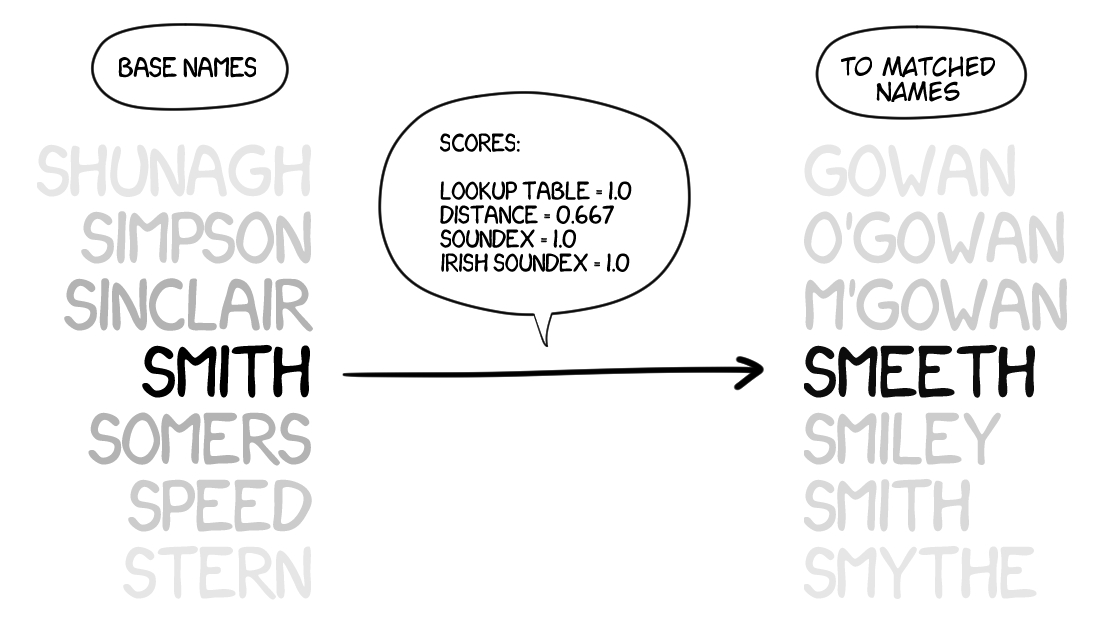
\includegraphics[width=11cm]{gfx/base_tmn}
\caption[\emph{Base name} `SMITH' comparing to \emph{to-match name} `SMEETH'.]{\emph{Base name}
`SMITH' comparing to \emph{to-match name} `SMEETH'. \\
Scores of each matching algorithms
are presented in the bubble above the arrow.}
\label{fig:base_tmn}
\end{figure}

Figure \ref{fig:base_tmn} shows a snapshot of an attempt to match between
\emph{base name} `SMITH' against \emph{to-match name} `SMEETH'.
\emph{Similarity score} for each matching algorithms have been calculated.
So the next step is to match current \emph{base name}, `SMITH',
against next \emph{to-match name}, `SMILEY'.

Once \emph{base name} `SMITH' completes all \emph{to-match name}\textquotesingle s in their list,
the system then process to the next \emph{base name}, `SOMERS', and start over
the matching process against the whole \emph{to-match name} list again, from
start to the end.

\section{Weighting matching algorithms}

We realised that, for matching names, each matching algorithms
should not be treat as all the same priority. For example, for Irish names,
it would be better if we favour \emph{Irish soundex} over the
traditional \emph{Soundex}, because it produces more accurate result.

By this idea we also implement \emph{weight} for each matching algorithm.
We will suggest initial values, but also allow client to change these values.
Table \ref{table:weights} states these initial weights.

\begin{table}[H]
  \myfloatalign
  \setlength{\tabcolsep}{0.3cm}
  \begin{tabular}{c c}
    \toprule
    \tableheadline{Matching algorithm} & \tableheadline{Weight} \\
    \midrule
    Levenshtein distance & 1 \\
    Soundex & 3 \\
    Irish soundex & 6 \\
    Lookup table & 10 \\
    \bottomrule
  \end{tabular}
  \caption{Matching algorithm weights.}
  \label{table:weights}
\end{table}

Usage and calculation of this weighting will be described in more detail
in the next section (\ref{sec:actualsys}).

\section{Actual system}
\label{sec:actualsys}

Following our basic idea from previous sections, we then design the
architecture of our system.

\begin{figure}[H]
\centering
\captionsetup{justification=centering}
\makebox[\textwidth][c]{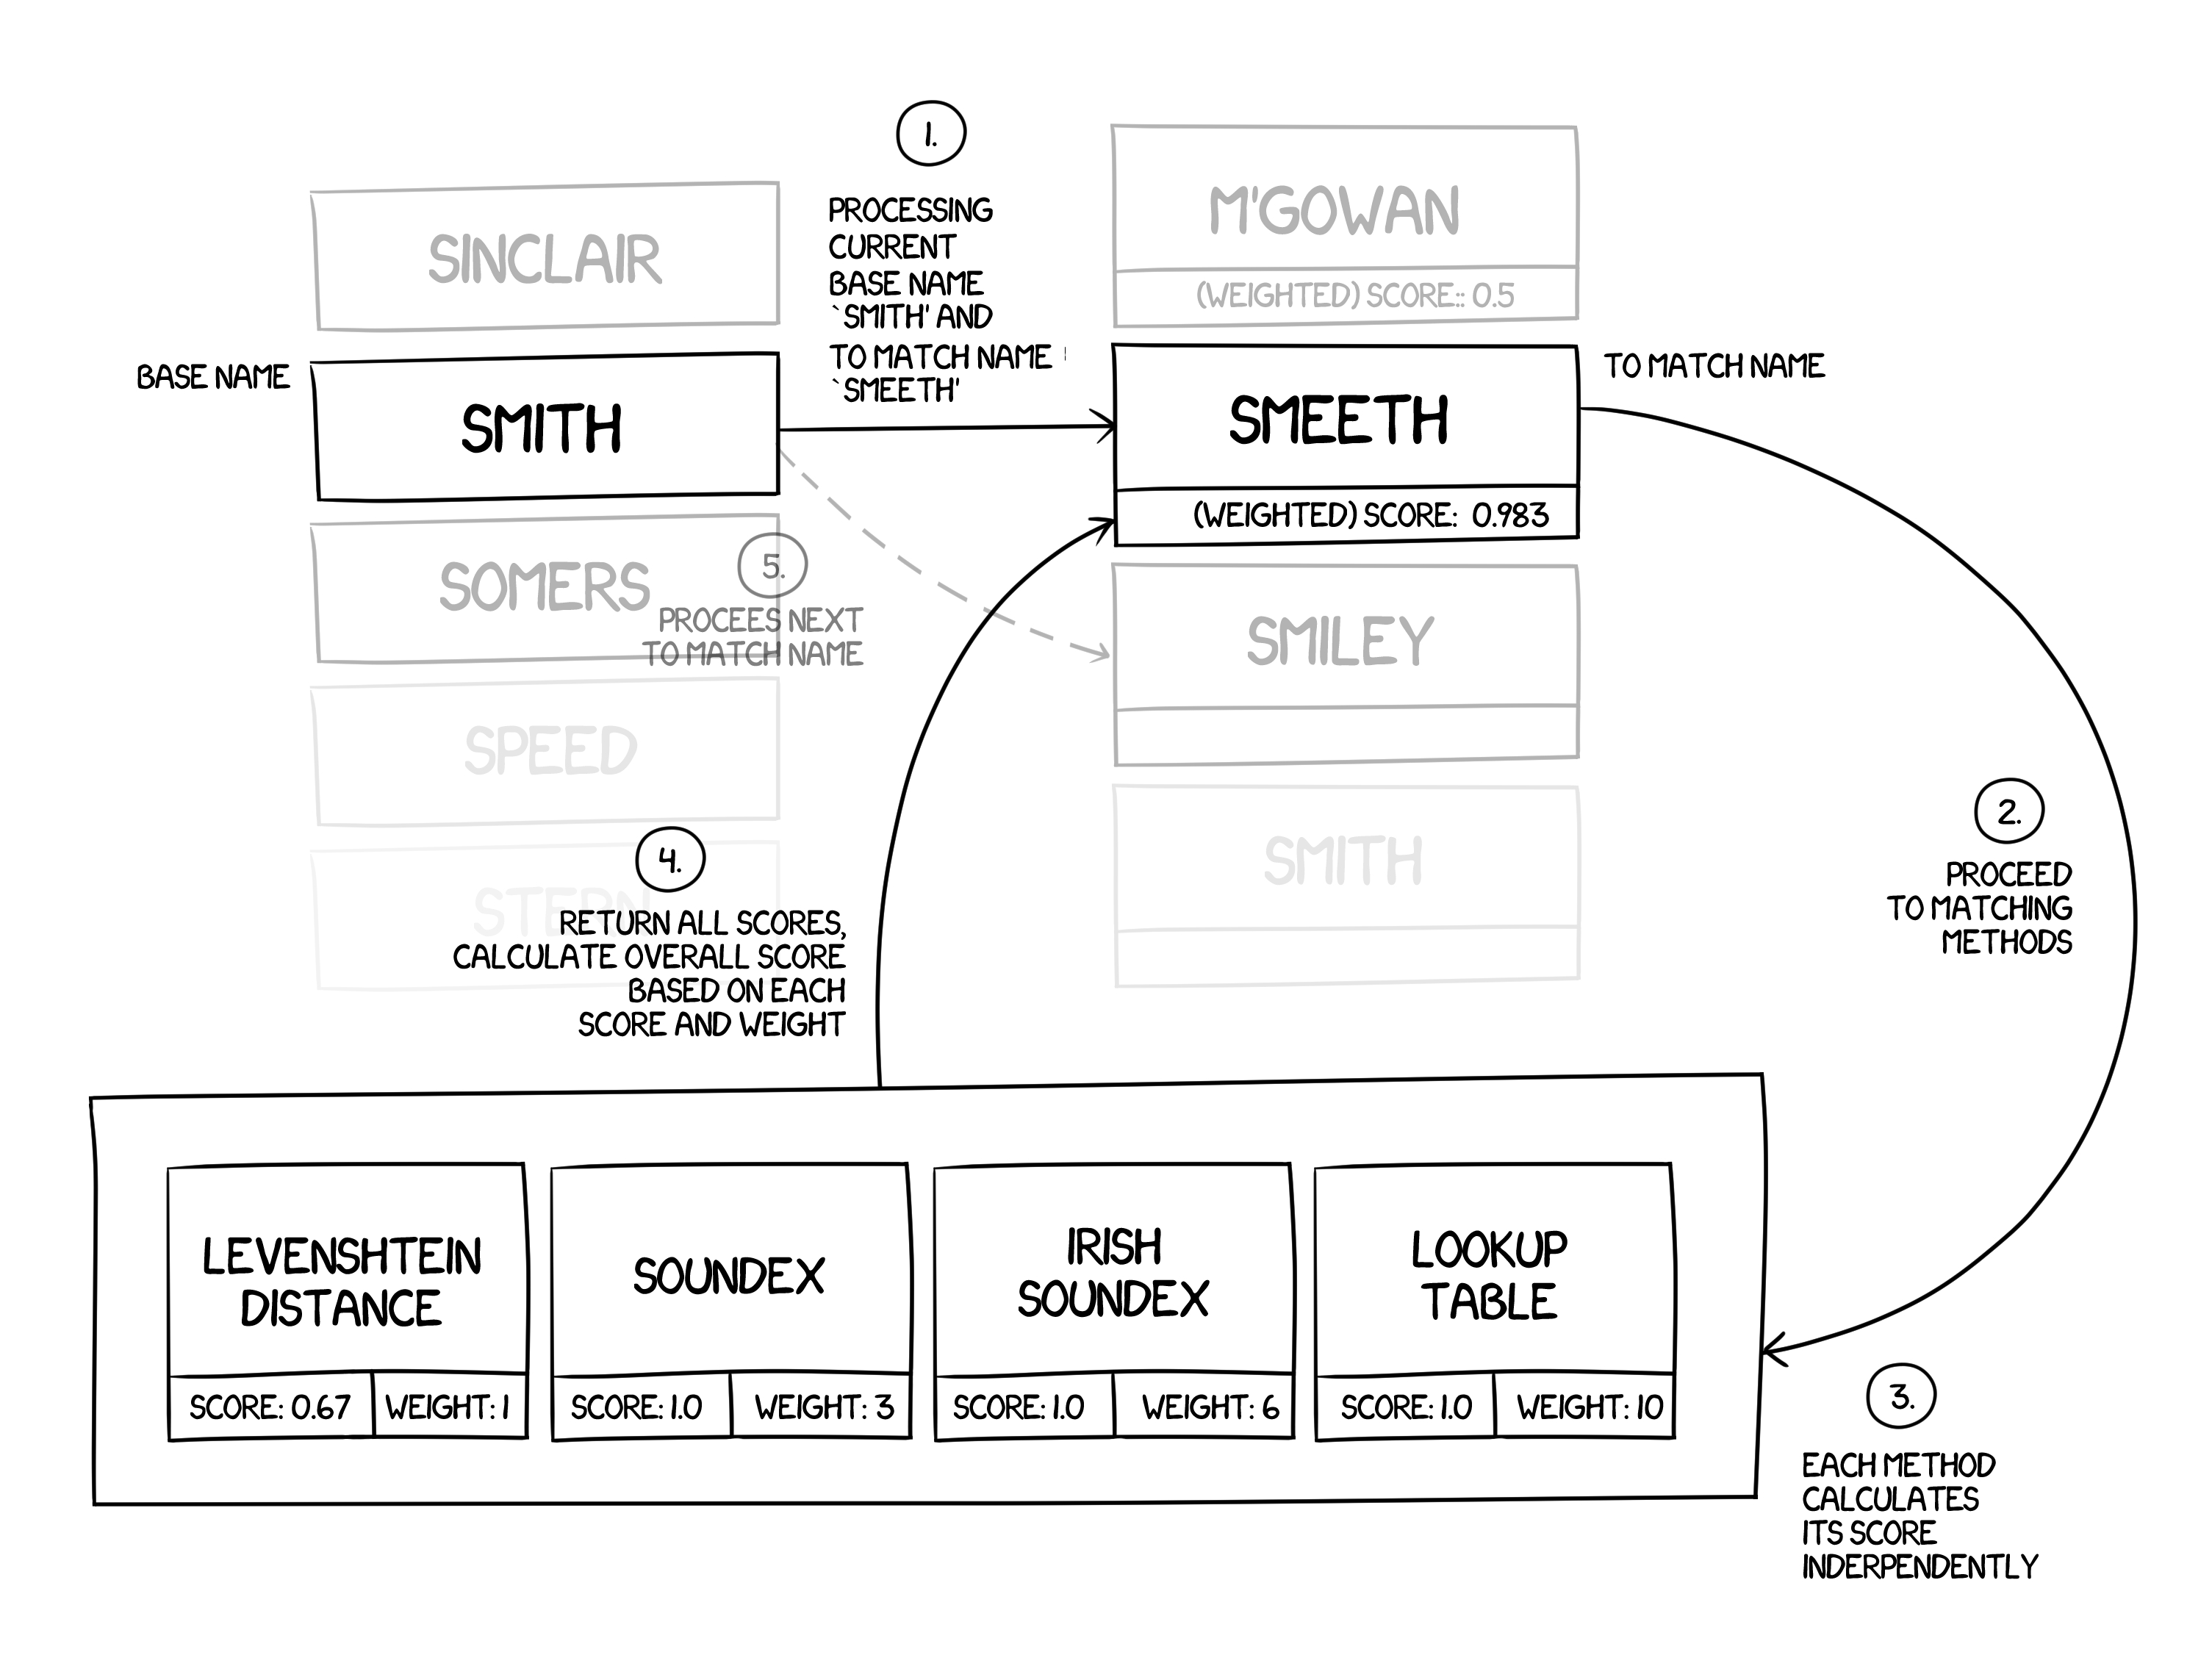
\includegraphics[width=16cm]{gfx/overall}}
\caption{Overall architecture.}
\label{fig:overall}
\end{figure}

\section{MVC}

% \lipsum[3]

\section{Web Interface}

% \lipsum[4]

\section{Web Service}

% \lipsum[5]
